\section{Tasks, Data, and Evaluation}
\label{app:protocol}

\subsection{The Reported Fourteen-Task Suite}
The completed studies use the migrated DB0 v0.6 demonstration pool and its
fourteen-task evaluation suite. Table~\ref{tab:tasks} lists the task identifiers
used in the result arrays. The task-balanced
score includes every task, including zero-success conditions.

\begin{table*}[!t]
\centering\fontsize{9}{11}\selectfont
\setlength{\tabcolsep}{4pt}
\renewcommand{\arraystretch}{1.13}
\caption{Native success conditions in the reported fourteen-task suite.
Thresholds come from the evaluator source and task configurations bound to the
accepted FUTURE0, BASE2, and HISTORY1 packages. A task must pass its preceding
stages and avoid terminal failures. All tasks run at 20\,Hz with a 2\,ms physics
step; durations below refer to physical time. COM denotes center of mass.}
\label{tab:tasks}
\begin{tabularx}{\textwidth}{@{}p{0.19\textwidth}Xp{0.07\textwidth}@{}}
\toprule
Task & Ordered success conditions & Limit \\
\midrule
grasp;\newline t1\_belt, t1\_xyz,\newline t1\_so3, t1\_occ
& Approach within 0.10\,m; bilateral fingerpad contact for 0.05\,s; collision-geometry
bottom at least 0.05\,m above support; retain contact and clearance for 0.50\,s.
T1 adds conveyor drive, translation, rotation, or a physical occluder.
SO3 has no additional success-angle threshold; unsafe occluder contact terminates OCC.
& 160 steps\newline 8\,s \\
t2\_trans
& Approach within 0.10\,m. Entire object collision geometry inside the receptacle:
planar clearance and floor gap both $\geq-0.002$\,m, top no higher than the opening.
Release requires an opening command $<-0.5$ and no fingerpad contact.
Relative linear/angular speeds $\leq0.08$\,m/s and $0.8$\,rad/s for 0.10\,s,
followed by a 0.50\,s stable dwell.
& 200\newline 10\,s \\
t2\_se3
& Approach within 0.05\,m and 0.12\,rad. Full T-shaped containment:
planar clearance $\geq0.002$\,m, floor gap in $[-0.002,0.002]$\,m,
tilt $\leq0.05$\,rad, top below opening.
After release, relative speeds $\leq0.02$\,m/s and $0.04$\,rad/s
for 0.10\,s, then a 0.50\,s dwell. The 0.12\,rad gate applies to approach.
& 200\newline 10\,s \\
t3\_phase
& Start with the native pre-grasp. Phase alignment: distance $\leq0.090$\,m and
loop-direction error $\leq0.20$\,rad. Enter within 0.030\,m at progress $\leq0.15$;
reach historical maximum progress $\geq0.60$, then $\geq0.85$ and endpoint
distance $\leq0.055$\,m.
& 420\newline 21\,s \\
t3\_full
& Acquire the wand with bilateral contact for 0.05\,s, then complete the phase
stages above. In a later sample, retain current progress $\geq0.85$ and move
at least 0.045\,m from both path and endpoint. Finally open ($<-0.5$)
with no fingerpad contact. Releasing before exit fails.
& 640\newline 32\,s \\
t4\_sphere
& Approach within 0.10\,m; first qualifying contact after ramp exit; any tray contact before success
fails. Bilateral hold for nominal 25\,ms (12 physics samples, 24\,ms).
Raise COM by 0.05\,m from its height when the bilateral-hold criterion is first met, and retain
contact and height for 0.50\,s.
& 120\newline 6\,s \\
t4\_sphere\_tabletop;\newline t4\_slider
& Approach within 0.10\,m; contact after ramp exit, while supported, in the capture region, and moving
at planar speed $\geq0.08$\,m/s. Bilateral hold for 0.05\,s, COM lift
$\geq0.05$\,m from the first attainment of that hold criterion, then contact and height for 0.50\,s.
& 120\newline 6\,s \\
t4\_can
& Same supported-capture sequence. Before first fingerpad contact, a can-axis
absolute dot product with vertical $>0.45$ fails as unstable tipping.
The configuration does not require a transverse closing axis.
& 120\newline 6\,s \\
t5\_replan
& Exactly one selected-side impact group completes before robot contact.
At 30\,ms after the physical impact-end timestamp, branch-signed lateral speed $\geq0.035$\,m/s and yaw rate
$\geq0.35$\,rad/s. Approach within 0.10\,m; bilateral hold with grasp-axis
error $\leq18^\circ$ for 0.05\,s; COM lift $\geq0.05$\,m from the first
attainment of that hold criterion and stable hold
for 0.50\,s. Impact-group lag is 12\,ms and maximum contact is 0.10\,s.
& 120\newline 6\,s \\
\bottomrule
\end{tabularx}
\end{table*}


\begin{figure*}[t]
\centering
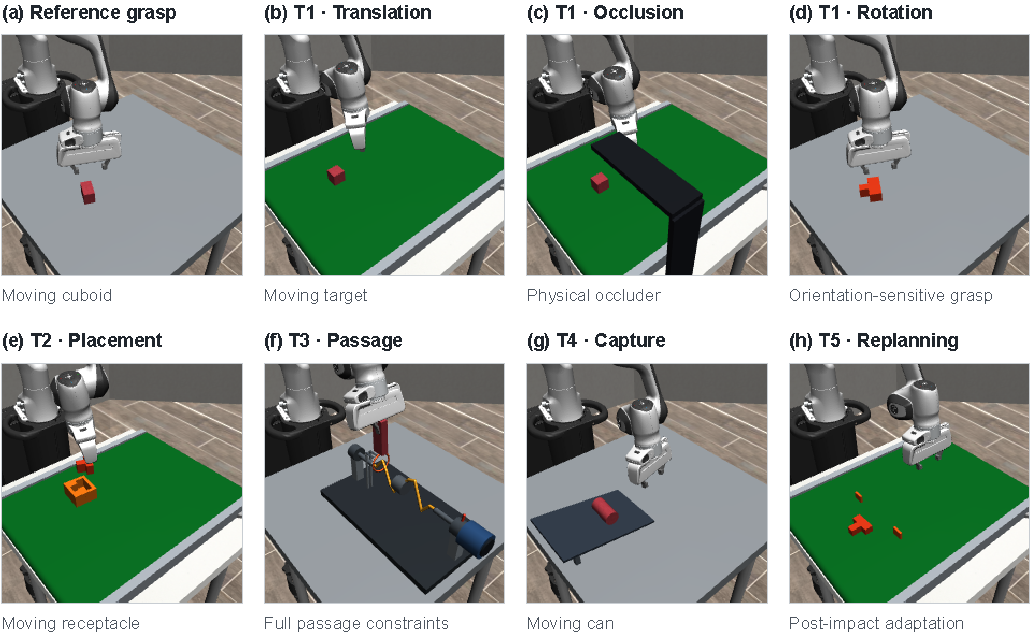
\includegraphics[width=\textwidth]{benchmark_task_examples.pdf}
\caption{Recorded benchmark observations. Eight examples cover reference
grasping; T1 translation, physical occlusion, and orientation-sensitive grasping;
T2 moving-receptacle placement; T3 constrained passage; T4 capture; and
T5 post-impact adaptation. For each displayed task, the lowest state index
in the accepted DEV84 manifest supplies the final observed, uncropped
$224\times224$ agentview RGB. Labels identify task conditions; the snapshots
illustrate appearance and geometry, while task outcomes are reported separately.
Table~\ref{tab:tasks} lists all fourteen tasks.}
\label{fig:benchmark_tasks}
\end{figure*}

The common training pool has 11,200 episodes, 800 per task. The internal
representation screen uses 350 validation episodes; adapted systems retain
their own validation settings (including 1,400 for DreamVLA/OpenWAM).
The future screen samples 160,416 chunks per epoch. Stored episode
count and effective chunk exposure measure different aspects of training.
Later fresh-data production retains its own data identity and does not
retroactively change the source of these results. Motion-only P0 prediction
has no corresponding action-learning score in the fourteen-task table.

Success is read from the native task evaluator after its ordered physical
requirements (Table~\ref{tab:tasks}). The accepted FUTURE0, BASE2, and HISTORY1
packages reference the same archived evaluator source, task configurations,
and fourteen-suite scenario manifest. We recover the definitions from that
archive. Success is checked at each 2\,ms physics step. Interrupted continuous
conditions reset their counters. For T2, the sample completing the low-relative-motion
counter also starts the stable-dwell counter; the two durations should not
be added as an exact 0.600\,s requirement.

\paragraph{Terminal events.}
The native result mapping groups events into five categories:
\emph{invalid} (invalid state);
\emph{boundary} (workspace or downstream exit, drop, expired goal window);
\emph{safety} (unsafe contact, excessive rim impulse, wire contact, stage block,
release impulse, early robot contact, tray or gripper--support contact,
striker trap);
\emph{task violation} (blocked driver, release outside the goal, path deviation
or backtracking, premature release, stopping/deflecting without capture,
unstable tipping, missing/extra impact, wrong striker contact, or insufficient
outgoing motion change);
and \emph{timeout}. These categories describe evaluator outcomes.

There is no global priority among categories. Each family selects the first
terminal event in its physics-step evaluation order and preserves that result.
Grasp checks invalid state, workspace exit, downstream exit, and drop before
success, then timeout. T1 inserts unsafe occluder contact after invalid state.
T2 checks invalid state, rim impulse $>0.10$\,N\,s, drop, goal-window expiry,
and release outside the goal before success and timeout.
T3 checks invalid state, stage block, drop, workspace exit, wire contact,
premature release, path deviation, and backtracking before success and timeout.
Wire failure uses impulse $>0.020$\,N\,s or penetration $>0.004$\,m for more
than two consecutive steps; path deviation is $>0.030$\,m for 0.050\,s,
and backtracking exceeds 0.05 relative to maximum progress.

T4 checks invalid state, release impulse $>0.002$\,N\,s, unsafe ramp contact,
unsupported tray contact, can tipping, early-contact/boundary branches,
and invalid supported capture before success and timeout.
A target that has exited the ramp, remains in contact with the downstream
support, and has no fingerpad contact at speed $\leq0.03$\,m/s for 0.25\,s
fails as stopping/deflecting only.
T5 checks invalid state, unsafe contact, early robot contact, wrong striker,
extra impact/striker trap, insufficient outgoing change, and boundary events
before success. At the horizon, zero completed impacts yields missing selected
impact; otherwise the result is timeout.

\subsection{Scenario Sampling and Replay}
\begin{table*}[!t]
\centering\fontsize{9}{11}\selectfont
\setlength{\tabcolsep}{4pt}
\renewcommand{\arraystretch}{1.12}
\caption{Historical validation proposal ranges. Length, linear velocity, angle,
and angular velocity use m, m/s, rad, and rad/s unless marked otherwise.
Positions are in world coordinates except the stated ramp-local offsets.
Continuous intervals are uniform proposals; discrete choices are equiprobable
before feasibility checks. Evaluation replays the stored accepted scenarios,
whose distribution need not remain uniform. Harmonic centers are not initial positions.}
\label{tab:task_sampling}
\begin{tabularx}{\textwidth}{@{}p{0.18\textwidth}p{0.34\textwidth}X@{}}
\toprule
Task & Initial-state proposal & Motion or event parameters \\
\midrule
grasp & Harmonic center $c_x\in[-.08,.08]$, $c_y\in[-.26,-.19]$, $z=.822$;
yaw $[-1.1,1.1]$.
& $v_y\in[.025,.125]$, $A_x\in[.015,.035]$, $f_x\in[.3,.7]$\,Hz;
$\omega_z\in[-1.2,1.2]$. \\
t1\_belt & Target $x\in[-.08,.08]$, $y\in[-.26,-.18]$, $z=.822$;
identity orientation, zero initial twist.
& Belt $v_y\in[.04,.10]$. \\
t1\_occ & Same target proposal as Belt; canopy at $(.322,-.29,1.20)$.
& Same belt range; clearance parameter .20; physical occlusion. \\
t1\_xyz & Harmonic center $c_x\in[-.025,.025]$, $c_y\in[-.24,-.20]$, $z=.818$;
yaw $[-.35,.35]$.
& $v_y\in[.04,.09]$, $A_x\in[0,.03]$, $f_x\in[.25,.65]$\,Hz; $\omega_z=0$. \\
t1\_so3 & Same as XYZ.
& Same translation; $\omega_z\in[-1.2,-.4]\cup[.4,1.2]$, equal sign probabilities. \\
t2\_trans & Goal $x\in[-.13,-.08]$, $y\in[-.18,-.12]$, $z=.825$; fixed orientation.
& Goal $v_y\in[.03,.06]$; no rotation. \\
t2\_se3 & Same goal $x,y$ range, $z=.804$; yaw $[-.3,.3]$.
& Goal $v_y\in[.03,.06]$;
$\omega_z\in[-.25,-.08]\cup[.08,.25]$, equal sign probabilities. \\
t3\_phase & Wand $x,y\in[-.03,.03]$, $z=.870$, yaw $[0,2\pi]$;
wire phase $[-.25,.35]$.
& Wire center $(.10,-.02,.94)$; world-X rotation
$\omega_x=-\{2.5,3,\ldots,7.5\}^{\circ}$/s (11 equal-probability values). \\
t3\_full & Wand at $(-.05,-.02,1.04)$ with identity orientation;
same wire phase range.
& Same wire rotation; cradle and release requirement enabled. \\
t4\_sphere & Ramp-local offsets: lateral $[-.015,.015]$, longitudinal/normal
$(-.145,.030)$; lip $(.06,-.02,1.10)$.
& Gravity-driven from rest; gate release at tick 0; slope $[5,15]^\circ$;
target/ramp sliding friction $[.7,.9]$; unsupported capture. \\
t4\_sphere\_tabletop & Lateral $[-.015,.015]$, longitudinal/normal
$(-.124,.034)$; lip $(0,-.06,.808)$.
& Same slope and release; target/ramp friction $[.7,.9]$, table friction .35. \\
t4\_slider & Lateral $[-.015,.015]$, longitudinal/normal $(-.129,.024)$;
supported ramp.
& Same slope and release; target/ramp friction $[.025,.045]$,
table friction $[.012,.018]$. \\
t4\_can & Lateral $[-.010,.010]$, ramp-axis yaw $[-4,4]^\circ$;
longitudinal position follows gate geometry and oriented can extent.
& Same slope and release; target/ramp friction $[.25,.45]$,
table friction $[.09,.15]$. \\
t5\_replan & $x\in[-.005,.005]$, $y=-.29$, $z=.812$;
yaw $[-.08,.08]$; zero initial twist.
& Belt $v_y\in[.12,.14]$; equal-probability left/right striker triggered at
$y=-.13$; stroke .098, pulse .35\,s, actuator scale $[1,1.1]$,
force cap 4\,N; command delay 50\,ms. \\
\bottomrule
\end{tabularx}
\end{table*}

The historical E7/agentview recipes specify proposal ranges
(Table~\ref{tab:task_sampling}). Continuous min--max fields use uniform draws
from NumPy PCG64; discrete choices are equiprobable before physical-feasibility
checks. Evaluation loads each accepted scene's complete stored ScenarioSpec
and does not resample its parameters.
For harmonic translation,
\[
p(t)=c+(0,v_y,0)t+(A_x\sin(2\pi f_xt+\phi),0,0),
\]
where $\phi\sim U[-\pi,\pi]$. Thus $c$ differs from the initial position by
the phase-dependent offset. T4 targets start at zero linear/angular velocity
and evolve under free dynamics; no constant target speed is prescribed.
Their slope is continuously sampled from $[5,15]^\circ$.
Ramp-local offsets use the ramp center as origin and lateral, downhill,
and normal axes: $p_{\rm world}=c_{\rm ramp}+R_x(-\alpha)p_{\rm offset}$.
The center is derived from the exit lip and ramp half-size; offsets are
not added directly to the lip.
T2-SE3 training uses $\omega_z\sim U[-.25,.25]$; validation excludes
$(-.08,.08)$. The other thirteen tasks share train/validation proposal recipes.

Occlusion acceptance requires at least eight initially visible frames with
visible fraction $\geq.95$, ten to sixty fully occluded frames
(fraction $\leq.05$, lasting 0.5--3.0\,s), and at least three reappearance
frames with fraction $\geq.8$. These are acceptance criteria, not independent
sampling variables. For example, the accepted OCC scenes have belt speeds
0.059588--0.099852\,m/s within the wider proposal interval.
Accepted source seeds can have gaps; a consecutive seed range does not
reconstruct the scene set.

All 1,400 stored scenarios share the robot joint initialization
\[
\begin{aligned}
q_0={}&[0,\ .19634954,\ 0,\ -2.61799388,\\
      &0,\ 2.94159265,\ .78539816]\ {\rm rad},
\end{aligned}
\]
and finger positions $(.020833,-.020833)$\,m.
T4 additionally stores a temporary preparation-target pose with
$x,y\sim U[-.03,.03]$ and yaw $U[0,2\pi]$, distinct from the release state.

The evaluator source stores recipes in \path{configs/scenarios/}
and task bindings in \path{configs/tasks/}; the generation entry point is
\path{se3_wam_benchmark/cli/generate_scenarios.py}.
The evaluation payload contains the concrete
\path{evaluation_reference/scenes/validation.jsonl} and fourteen
\path{evaluation_reference/scenes/suites/sr_<task>.yaml} files.
Each suite uses one repeat and filters the shared manifest by task.
These files, with the stored scenario IDs and source seeds, define the
replay set used for the paired comparisons.

The accompanying local material package at
\path{results/replay_materials/} contains the archived evaluator, task and
sampling configurations, all accepted scenarios, and both ordered selections.
Portable copies change only execution paths; originals are retained.
The archived manifest parser reads all 1,400 scenarios without changing their
scientific fields, and the task/configuration loaders read all fourteen
definitions. The supplied checker also verifies disjoint partitions, identities,
seeds, and asset references. These checks parse the materials; physics and
policy replay require the additional runtime and model assets listed in the
package instructions.

\subsection{Partitions and Statistical Interpretation}
The 140-scene development set has ten scenes per task. Its disjoint complement
has ninety per task, totaling 1,260. The future screen reports the two
partitions separately. The system-reference study also keeps them separate.
The combination screen explicitly selects on all 1,400 scenes while retaining
both component counts. Thus its selection score includes development data,
and the 1,260 complement is now part of the project's development evidence.
Neither membership disjointness nor a different rollout seed makes it a final
blind test.

The future study uses each condition's own fourth-epoch endpoint and one
training seed. Across arms, the scene, source seed, and inference seed are
paired. There are 18,900 accepted outcomes, 1,260 per arm; missing scenes and
infrastructure-error exclusions are zero. Inference seeds span
20261058--20262317 for the designated selection indices. Matching an inference
seed specifies rollout randomness but does not imply that unlike training
graphs consumed identical random-number sequences.

For two policies on the same scenes, let $b$ count candidate successes/reference
failures and $c$ candidate failures/reference successes. Then
\begin{equation}
 \Delta\mathrm{SR}=100(b-c)/1260
\end{equation}
in percentage points. The report uses the exact two-sided McNemar test on
discordant pairs. Fourteen comparisons to P00 and thirteen to P03 form the
twenty-seven-comparison family; adjusted values use
$\min(1,27p)$. The 378 task-level comparisons remain exploratory.

We additionally compute 95\% pointwise percentile intervals by resampling paired
scenes within each task. For every replicate, each task retains ninety pairs
(one hundred in the combination study), and the fourteen task differences are
averaged with equal weights. Sampling a multinomial from each task's four
paired outcome counts is equivalent to resampling its binary scene pairs.
We use 100,000 replicates and the 2.5th/97.5th percentiles with linear interpolation.
The generator is NumPy 2.3.5 PCG64; seeds are 20261017 plus the zero-based
lexicographic comparison index for the twenty-seven future contrasts,
and 20261017/20261018 for I versus F/E. The post-hoc I--E analysis excluding
phase passage retains thirteen tasks with seed 20261019.
Tasks are processed in lexicographic order.
These intervals condition on the trained checkpoints and fixed task mixture;
they do not include training-seed variation or candidate-selection uncertainty.
They are not simultaneous intervals; the corrected McNemar family above
remains the basis for the overall future-screen comparisons.

\subsection{Inputs and Time}
The completed future screen uses one current fixed-camera RGB view, exact
depth/camera geometry, robot-state history, and privileged object information.
A simulator field stored beside an image is not automatically a deployable
sensor observation. Future target states and label-validity masks supervise
their respective branches and are excluded from the action condition.
A current-object-pose oracle and a future oracle are distinct information
conditions.

Physical high-level steps are separated by 50\,ms. All one hundred T5 scenarios
use a one-step command delay (50\,ms); the other thirteen tasks use zero.
The native action queue returns a zero command until the delay elapses,
then applies the oldest queued command. Forecast labels cover
50--400\,ms relative to the source observation. Synchronous evaluation pauses
the environment for policy computation, so it cannot measure the consequence
of wall-clock observation age. Later fixed-delay and real-delay evaluations
must retain their own time traces and report whether physics continues while
the policy computes. Future labels follow the demonstration's recorded
geometry under its executed actions. The current validity masks check
geometric support, projection, and visibility. They do not establish that the
same post-contact future remains valid for an alternative candidate action.
Action-consistent label support is \placeholder{pending for online generation}.
